\documentclass{standalone}
\usepackage{tikz}
\usetikzlibrary{patterns, positioning}

\begin{document}
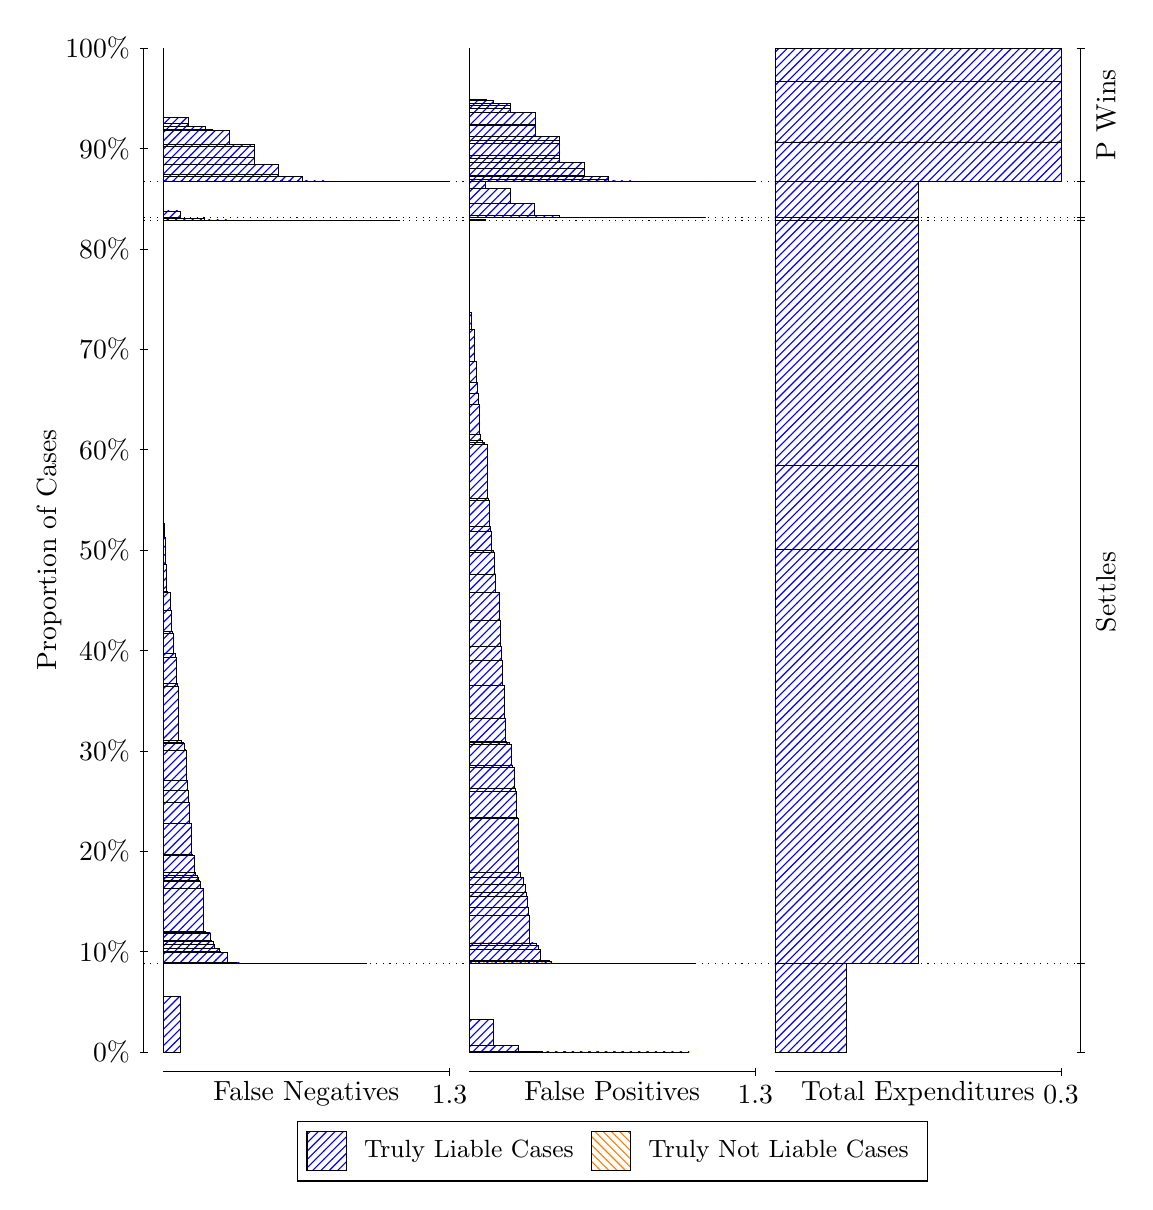
\begin{tikzpicture}
\draw[black, very thin] (1.5,1.75) -- (1.5,14.5);
\node[rotate=90, anchor=center] at (0.3, 8.125) {Proportion of Cases};
\draw[black, very thin] (1.45,1.75) -- (1.55,1.75);
\node[anchor=east] at (1.45, 1.75) {0\%};
\draw[black, very thin] (1.45,3.025) -- (1.55,3.025);
\node[anchor=east] at (1.45, 3.025) {10\%};
\draw[black, very thin] (1.45,4.3) -- (1.55,4.3);
\node[anchor=east] at (1.45, 4.3) {20\%};
\draw[black, very thin] (1.45,5.575) -- (1.55,5.575);
\node[anchor=east] at (1.45, 5.575) {30\%};
\draw[black, very thin] (1.45,6.85) -- (1.55,6.85);
\node[anchor=east] at (1.45, 6.85) {40\%};
\draw[black, very thin] (1.45,8.125) -- (1.55,8.125);
\node[anchor=east] at (1.45, 8.125) {50\%};
\draw[black, very thin] (1.45,9.4) -- (1.55,9.4);
\node[anchor=east] at (1.45, 9.4) {60\%};
\draw[black, very thin] (1.45,10.675) -- (1.55,10.675);
\node[anchor=east] at (1.45, 10.675) {70\%};
\draw[black, very thin] (1.45,11.95) -- (1.55,11.95);
\node[anchor=east] at (1.45, 11.95) {80\%};
\draw[black, very thin] (1.45,13.225) -- (1.55,13.225);
\node[anchor=east] at (1.45, 13.225) {90\%};
\draw[black, very thin] (1.45,14.5) -- (1.55,14.5);
\node[anchor=east] at (1.45, 14.5) {100\%};

\draw[black, very thin] (13.4,1.75) -- (13.4,14.5);
\draw[black, very thin] (13.35,1.75) -- (13.45,1.75);
\node[anchor=west] at (13.35, 1.75) {};
\draw[black, very thin] (13.35,2.8721) -- (13.45,2.8721);
\node[anchor=west] at (13.35, 2.8721) {};
\draw[black, very thin] (13.35,12.309) -- (13.45,12.309);
\node[anchor=west] at (13.35, 12.309) {};
\draw[black, very thin] (13.35,12.349) -- (13.45,12.349);
\node[anchor=west] at (13.35, 12.349) {};
\draw[black, very thin] (13.35,12.803) -- (13.45,12.803);
\node[anchor=west] at (13.35, 12.803) {};
\draw[black, very thin] (13.35,14.5) -- (13.45,14.5);
\node[anchor=west] at (13.35, 14.5) {};

\draw[black, very thin, pattern color=blue, pattern=north east lines] (1.75,1.75) rectangle (1.9596,2.4561);
\draw[black, very thin, pattern color=orange, pattern=north west lines] (1.75,2.4561) rectangle (1.75,2.4561);
\draw[black, very thin, pattern color=blue, pattern=north east lines] (1.75,2.4561) rectangle (1.75,2.8721);
\draw[black, very thin, pattern color=blue, pattern=north east lines] (1.75,2.8721) rectangle (4.3353,2.8721);
\draw[black, very thin, pattern color=blue, pattern=north east lines] (1.75,2.8721) rectangle (4.1955,2.8721);
\draw[black, very thin, pattern color=blue, pattern=north east lines] (1.75,2.8721) rectangle (4.0558,2.8721);
\draw[black, very thin, pattern color=blue, pattern=north east lines] (1.75,2.8721) rectangle (4.0247,2.8721);
\draw[black, very thin, pattern color=blue, pattern=north east lines] (1.75,2.8721) rectangle (3.916,2.8721);
\draw[black, very thin, pattern color=blue, pattern=north east lines] (1.75,2.8721) rectangle (3.885,2.8721);
\draw[black, very thin, pattern color=blue, pattern=north east lines] (1.75,2.8721) rectangle (3.7763,2.8721);
\draw[black, very thin, pattern color=blue, pattern=north east lines] (1.75,2.8721) rectangle (3.7452,2.8721);
\draw[black, very thin, pattern color=blue, pattern=north east lines] (1.75,2.8721) rectangle (3.7142,2.8721);
\draw[black, very thin, pattern color=blue, pattern=north east lines] (1.75,2.8721) rectangle (3.6365,2.8721);
\draw[black, very thin, pattern color=blue, pattern=north east lines] (1.75,2.8721) rectangle (3.6055,2.8721);
\draw[black, very thin, pattern color=blue, pattern=north east lines] (1.75,2.8721) rectangle (3.5744,2.8721);
\draw[black, very thin, pattern color=blue, pattern=north east lines] (1.75,2.8721) rectangle (3.4968,2.8721);
\draw[black, very thin, pattern color=blue, pattern=north east lines] (1.75,2.8721) rectangle (3.4657,2.8721);
\draw[black, very thin, pattern color=blue, pattern=north east lines] (1.75,2.8721) rectangle (3.4347,2.8721);
\draw[black, very thin, pattern color=blue, pattern=north east lines] (1.75,2.8721) rectangle (3.4036,2.8721);
\draw[black, very thin, pattern color=blue, pattern=north east lines] (1.75,2.8721) rectangle (3.3571,2.8721);
\draw[black, very thin, pattern color=blue, pattern=north east lines] (1.75,2.8721) rectangle (3.326,2.8721);
\draw[black, very thin, pattern color=blue, pattern=north east lines] (1.75,2.8721) rectangle (3.2949,2.8721);
\draw[black, very thin, pattern color=blue, pattern=north east lines] (1.75,2.8721) rectangle (3.2639,2.8721);
\draw[black, very thin, pattern color=blue, pattern=north east lines] (1.75,2.8721) rectangle (3.2173,2.8721);
\draw[black, very thin, pattern color=blue, pattern=north east lines] (1.75,2.8721) rectangle (3.1863,2.8721);
\draw[black, very thin, pattern color=blue, pattern=north east lines] (1.75,2.8721) rectangle (3.1552,2.8721);
\draw[black, very thin, pattern color=blue, pattern=north east lines] (1.75,2.8721) rectangle (3.1241,2.8721);
\draw[black, very thin, pattern color=blue, pattern=north east lines] (1.75,2.8721) rectangle (3.0931,2.8721);
\draw[black, very thin, pattern color=blue, pattern=north east lines] (1.75,2.8721) rectangle (3.0776,2.8722);
\draw[black, very thin, pattern color=blue, pattern=north east lines] (1.75,2.8722) rectangle (3.0465,2.8722);
\draw[black, very thin, pattern color=blue, pattern=north east lines] (1.75,2.8722) rectangle (3.0155,2.8722);
\draw[black, very thin, pattern color=blue, pattern=north east lines] (1.75,2.8722) rectangle (2.9844,2.8722);
\draw[black, very thin, pattern color=blue, pattern=north east lines] (1.75,2.8722) rectangle (2.9533,2.8722);
\draw[black, very thin, pattern color=blue, pattern=north east lines] (1.75,2.8722) rectangle (2.9378,2.8722);
\draw[black, very thin, pattern color=blue, pattern=north east lines] (1.75,2.8722) rectangle (2.9378,2.8722);
\draw[black, very thin, pattern color=blue, pattern=north east lines] (1.75,2.8722) rectangle (2.9068,2.8722);
\draw[black, very thin, pattern color=blue, pattern=north east lines] (1.75,2.8722) rectangle (2.8757,2.8779);
\draw[black, very thin, pattern color=blue, pattern=north east lines] (1.75,2.8779) rectangle (2.8447,2.878);
\draw[black, very thin, pattern color=blue, pattern=north east lines] (1.75,2.878) rectangle (2.8136,2.878);
\draw[black, very thin, pattern color=blue, pattern=north east lines] (1.75,2.878) rectangle (2.7981,2.8782);
\draw[black, very thin, pattern color=blue, pattern=north east lines] (1.75,2.8782) rectangle (2.7825,2.8782);
\draw[black, very thin, pattern color=blue, pattern=north east lines] (1.75,2.8782) rectangle (2.767,2.8805);
\draw[black, very thin, pattern color=blue, pattern=north east lines] (1.75,2.8805) rectangle (2.736,2.8805);
\draw[black, very thin, pattern color=blue, pattern=north east lines] (1.75,2.8805) rectangle (2.7049,2.8828);
\draw[black, very thin, pattern color=blue, pattern=north east lines] (1.75,2.8828) rectangle (2.6739,2.8831);
\draw[black, very thin, pattern color=blue, pattern=north east lines] (1.75,2.8831) rectangle (2.6583,2.8909);
\draw[black, very thin, pattern color=blue, pattern=north east lines] (1.75,2.8909) rectangle (2.6428,2.8909);
\draw[black, very thin, pattern color=blue, pattern=north east lines] (1.75,2.8909) rectangle (2.6273,2.8909);
\draw[black, very thin, pattern color=blue, pattern=north east lines] (1.75,2.8909) rectangle (2.6273,2.8913);
\draw[black, very thin, pattern color=blue, pattern=north east lines] (1.75,2.8913) rectangle (2.5962,2.8915);
\draw[black, very thin, pattern color=blue, pattern=north east lines] (1.75,2.8915) rectangle (2.5652,3.0104);
\draw[black, very thin, pattern color=blue, pattern=north east lines] (1.75,3.0104) rectangle (2.5341,3.0161);
\draw[black, very thin, pattern color=blue, pattern=north east lines] (1.75,3.0161) rectangle (2.5186,3.0179);
\draw[black, very thin, pattern color=blue, pattern=north east lines] (1.75,3.0179) rectangle (2.5031,3.0187);
\draw[black, very thin, pattern color=blue, pattern=north east lines] (1.75,3.0187) rectangle (2.4875,3.0222);
\draw[black, very thin, pattern color=blue, pattern=north east lines] (1.75,3.0222) rectangle (2.472,3.0235);
\draw[black, very thin, pattern color=blue, pattern=north east lines] (1.75,3.0235) rectangle (2.4565,3.0705);
\draw[black, very thin, pattern color=blue, pattern=north east lines] (1.75,3.0705) rectangle (2.4254,3.0706);
\draw[black, very thin, pattern color=blue, pattern=north east lines] (1.75,3.0706) rectangle (2.3944,3.1236);
\draw[black, very thin, pattern color=blue, pattern=north east lines] (1.75,3.1236) rectangle (2.3788,3.1586);
\draw[black, very thin, pattern color=blue, pattern=north east lines] (1.75,3.1586) rectangle (2.3633,3.1702);
\draw[black, very thin, pattern color=blue, pattern=north east lines] (1.75,3.1702) rectangle (2.3478,3.2631);
\draw[black, very thin, pattern color=blue, pattern=north east lines] (1.75,3.2631) rectangle (2.3323,3.2675);
\draw[black, very thin, pattern color=blue, pattern=north east lines] (1.75,3.2675) rectangle (2.3167,3.2676);
\draw[black, very thin, pattern color=blue, pattern=north east lines] (1.75,3.2676) rectangle (2.3167,3.2743);
\draw[black, very thin, pattern color=blue, pattern=north east lines] (1.75,3.2743) rectangle (2.2857,3.2787);
\draw[black, very thin, pattern color=blue, pattern=north east lines] (1.75,3.2787) rectangle (2.2546,3.8245);
\draw[black, very thin, pattern color=blue, pattern=north east lines] (1.75,3.8245) rectangle (2.2391,3.8328);
\draw[black, very thin, pattern color=blue, pattern=north east lines] (1.75,3.8328) rectangle (2.2236,3.9185);
\draw[black, very thin, pattern color=blue, pattern=north east lines] (1.75,3.9185) rectangle (2.208,3.9366);
\draw[black, very thin, pattern color=blue, pattern=north east lines] (1.75,3.9366) rectangle (2.1925,3.9731);
\draw[black, very thin, pattern color=blue, pattern=north east lines] (1.75,3.9731) rectangle (2.177,3.9939);
\draw[black, very thin, pattern color=blue, pattern=north east lines] (1.75,3.9939) rectangle (2.1615,4.0312);
\draw[black, very thin, pattern color=blue, pattern=north east lines] (1.75,4.0312) rectangle (2.1459,4.2534);
\draw[black, very thin, pattern color=blue, pattern=north east lines] (1.75,4.2534) rectangle (2.1149,4.2556);
\draw[black, very thin, pattern color=blue, pattern=north east lines] (1.75,4.2556) rectangle (2.0994,4.6583);
\draw[black, very thin, pattern color=blue, pattern=north east lines] (1.75,4.6583) rectangle (2.0838,4.9253);
\draw[black, very thin, pattern color=blue, pattern=north east lines] (1.75,4.9253) rectangle (2.0683,5.0698);
\draw[black, very thin, pattern color=blue, pattern=north east lines] (1.75,5.0698) rectangle (2.0528,5.2025);
\draw[black, very thin, pattern color=blue, pattern=north east lines] (1.75,5.2025) rectangle (2.0373,5.5858);
\draw[black, very thin, pattern color=blue, pattern=north east lines] (1.75,5.5858) rectangle (2.0217,5.6665);
\draw[black, very thin, pattern color=blue, pattern=north east lines] (1.75,5.6665) rectangle (2.0062,5.667);
\draw[black, very thin, pattern color=blue, pattern=north east lines] (1.75,5.667) rectangle (2.0062,5.686);
\draw[black, very thin, pattern color=blue, pattern=north east lines] (1.75,5.686) rectangle (1.9751,5.7085);
\draw[black, very thin, pattern color=blue, pattern=north east lines] (1.75,5.7085) rectangle (1.9441,6.399);
\draw[black, very thin, pattern color=blue, pattern=north east lines] (1.75,6.399) rectangle (1.9286,6.4278);
\draw[black, very thin, pattern color=blue, pattern=north east lines] (1.75,6.4278) rectangle (1.913,6.7572);
\draw[black, very thin, pattern color=blue, pattern=north east lines] (1.75,6.7572) rectangle (1.8975,6.812);
\draw[black, very thin, pattern color=blue, pattern=north east lines] (1.75,6.812) rectangle (1.882,7.0636);
\draw[black, very thin, pattern color=blue, pattern=north east lines] (1.75,7.0636) rectangle (1.8665,7.087);
\draw[black, very thin, pattern color=blue, pattern=north east lines] (1.75,7.087) rectangle (1.8509,7.3588);
\draw[black, very thin, pattern color=blue, pattern=north east lines] (1.75,7.3588) rectangle (1.8354,7.5907);
\draw[black, very thin, pattern color=blue, pattern=north east lines] (1.75,7.5907) rectangle (1.8043,7.5957);
\draw[black, very thin, pattern color=blue, pattern=north east lines] (1.75,7.5957) rectangle (1.7888,7.9459);
\draw[black, very thin, pattern color=blue, pattern=north east lines] (1.75,7.9459) rectangle (1.7733,8.2807);
\draw[black, very thin, pattern color=blue, pattern=north east lines] (1.75,8.2807) rectangle (1.7578,8.4584);
\draw[black, very thin, pattern color=orange, pattern=north west lines] (1.75,8.4584) rectangle (1.75,8.4584);
\draw[black, very thin, pattern color=blue, pattern=north east lines] (1.75,8.4584) rectangle (1.75,12.309);
\draw[black, very thin, pattern color=blue, pattern=north east lines] (1.75,12.309) rectangle (4.7545,12.309);
\draw[black, very thin, pattern color=blue, pattern=north east lines] (1.75,12.309) rectangle (4.4439,12.309);
\draw[black, very thin, pattern color=blue, pattern=north east lines] (1.75,12.309) rectangle (4.1334,12.309);
\draw[black, very thin, pattern color=blue, pattern=north east lines] (1.75,12.309) rectangle (3.8229,12.309);
\draw[black, very thin, pattern color=blue, pattern=north east lines] (1.75,12.309) rectangle (3.5123,12.309);
\draw[black, very thin, pattern color=blue, pattern=north east lines] (1.75,12.309) rectangle (3.2018,12.309);
\draw[black, very thin, pattern color=blue, pattern=north east lines] (1.75,12.309) rectangle (2.8912,12.31);
\draw[black, very thin, pattern color=blue, pattern=north east lines] (1.75,12.31) rectangle (2.5807,12.318);
\draw[black, very thin, pattern color=blue, pattern=north east lines] (1.75,12.318) rectangle (2.2702,12.337);
\draw[black, very thin, pattern color=blue, pattern=north east lines] (1.75,12.337) rectangle (1.9596,12.349);
\draw[black, very thin, pattern color=orange, pattern=north west lines] (1.75,12.349) rectangle (1.75,12.349);
\draw[black, very thin, pattern color=blue, pattern=north east lines] (1.75,12.349) rectangle (1.9596,12.431);
\draw[black, very thin, pattern color=orange, pattern=north west lines] (1.75,12.431) rectangle (1.75,12.431);
\draw[black, very thin, pattern color=blue, pattern=north east lines] (1.75,12.431) rectangle (1.75,12.803);
\draw[black, very thin, pattern color=blue, pattern=north east lines] (1.75,12.803) rectangle (5.3833,12.803);
\draw[black, very thin, pattern color=blue, pattern=north east lines] (1.75,12.803) rectangle (5.0728,12.803);
\draw[black, very thin, pattern color=blue, pattern=north east lines] (1.75,12.803) rectangle (4.7623,12.803);
\draw[black, very thin, pattern color=blue, pattern=north east lines] (1.75,12.803) rectangle (4.4517,12.803);
\draw[black, very thin, pattern color=blue, pattern=north east lines] (1.75,12.803) rectangle (4.4517,12.803);
\draw[black, very thin, pattern color=blue, pattern=north east lines] (1.75,12.803) rectangle (4.1412,12.803);
\draw[black, very thin, pattern color=blue, pattern=north east lines] (1.75,12.803) rectangle (4.1412,12.804);
\draw[black, very thin, pattern color=blue, pattern=north east lines] (1.75,12.804) rectangle (3.9238,12.804);
\draw[black, very thin, pattern color=blue, pattern=north east lines] (1.75,12.804) rectangle (3.8306,12.814);
\draw[black, very thin, pattern color=blue, pattern=north east lines] (1.75,12.814) rectangle (3.6132,12.814);
\draw[black, very thin, pattern color=blue, pattern=north east lines] (1.75,12.814) rectangle (3.6132,12.814);
\draw[black, very thin, pattern color=blue, pattern=north east lines] (1.75,12.814) rectangle (3.5201,12.865);
\draw[black, very thin, pattern color=blue, pattern=north east lines] (1.75,12.865) rectangle (3.3027,12.865);
\draw[black, very thin, pattern color=blue, pattern=north east lines] (1.75,12.865) rectangle (3.2095,12.896);
\draw[black, very thin, pattern color=blue, pattern=north east lines] (1.75,12.896) rectangle (3.2095,13.024);
\draw[black, very thin, pattern color=blue, pattern=north east lines] (1.75,13.024) rectangle (2.9922,13.024);
\draw[black, very thin, pattern color=blue, pattern=north east lines] (1.75,13.024) rectangle (2.9922,13.024);
\draw[black, very thin, pattern color=blue, pattern=north east lines] (1.75,13.024) rectangle (2.899,13.115);
\draw[black, very thin, pattern color=blue, pattern=north east lines] (1.75,13.115) rectangle (2.899,13.253);
\draw[black, very thin, pattern color=blue, pattern=north east lines] (1.75,13.253) rectangle (2.899,13.278);
\draw[black, very thin, pattern color=blue, pattern=north east lines] (1.75,13.278) rectangle (2.6816,13.278);
\draw[black, very thin, pattern color=blue, pattern=north east lines] (1.75,13.278) rectangle (2.6816,13.278);
\draw[black, very thin, pattern color=blue, pattern=north east lines] (1.75,13.278) rectangle (2.6816,13.278);
\draw[black, very thin, pattern color=blue, pattern=north east lines] (1.75,13.278) rectangle (2.5885,13.456);
\draw[black, very thin, pattern color=blue, pattern=north east lines] (1.75,13.456) rectangle (2.3711,13.456);
\draw[black, very thin, pattern color=blue, pattern=north east lines] (1.75,13.456) rectangle (2.3711,13.468);
\draw[black, very thin, pattern color=blue, pattern=north east lines] (1.75,13.468) rectangle (2.2779,13.469);
\draw[black, very thin, pattern color=blue, pattern=north east lines] (1.75,13.469) rectangle (2.2779,13.509);
\draw[black, very thin, pattern color=blue, pattern=north east lines] (1.75,13.509) rectangle (2.2779,13.509);
\draw[black, very thin, pattern color=blue, pattern=north east lines] (1.75,13.509) rectangle (2.0605,13.539);
\draw[black, very thin, pattern color=blue, pattern=north east lines] (1.75,13.539) rectangle (2.0605,13.544);
\draw[black, very thin, pattern color=blue, pattern=north east lines] (1.75,13.544) rectangle (2.0605,13.619);
\draw[black, very thin, pattern color=blue, pattern=north east lines] (1.75,13.619) rectangle (1.9674,13.62);
\draw[black, very thin, pattern color=blue, pattern=north east lines] (1.75,13.62) rectangle (1.9674,13.62);
\draw[black, very thin, pattern color=orange, pattern=north west lines] (1.75,13.62) rectangle (1.75,13.62);
\draw[black, very thin, pattern color=blue, pattern=north east lines] (1.75,13.62) rectangle (1.75,14.5);
\draw[black, very thin, pattern color=orange, pattern=north west lines] (5.6333,1.75) rectangle (8.4282,1.75);
\draw[black, very thin, pattern color=blue, pattern=north east lines] (5.6333,1.75) rectangle (8.4282,1.75);
\draw[black, very thin, pattern color=blue, pattern=north east lines] (5.6333,1.75) rectangle (8.1177,1.75);
\draw[black, very thin, pattern color=blue, pattern=north east lines] (5.6333,1.75) rectangle (7.8071,1.75);
\draw[black, very thin, pattern color=blue, pattern=north east lines] (5.6333,1.75) rectangle (7.4966,1.75);
\draw[black, very thin, pattern color=blue, pattern=north east lines] (5.6333,1.75) rectangle (7.186,1.75);
\draw[black, very thin, pattern color=blue, pattern=north east lines] (5.6333,1.75) rectangle (6.8755,1.7503);
\draw[black, very thin, pattern color=blue, pattern=north east lines] (5.6333,1.7503) rectangle (6.565,1.7579);
\draw[black, very thin, pattern color=blue, pattern=north east lines] (5.6333,1.7579) rectangle (6.2544,1.8357);
\draw[black, very thin, pattern color=blue, pattern=north east lines] (5.6333,1.8357) rectangle (5.9439,2.166);
\draw[black, very thin, pattern color=blue, pattern=north east lines] (5.6333,2.166) rectangle (5.6333,2.8721);
\draw[black, very thin, pattern color=orange, pattern=north west lines] (5.6333,2.8721) rectangle (8.4981,2.8721);
\draw[black, very thin, pattern color=blue, pattern=north east lines] (5.6333,2.8721) rectangle (8.4981,2.8721);
\draw[black, very thin, pattern color=orange, pattern=north west lines] (5.6333,2.8721) rectangle (8.3583,2.8721);
\draw[black, very thin, pattern color=blue, pattern=north east lines] (5.6333,2.8721) rectangle (8.3583,2.8721);
\draw[black, very thin, pattern color=orange, pattern=north west lines] (5.6333,2.8721) rectangle (8.2186,2.8721);
\draw[black, very thin, pattern color=blue, pattern=north east lines] (5.6333,2.8721) rectangle (8.2186,2.8721);
\draw[black, very thin, pattern color=blue, pattern=north east lines] (5.6333,2.8721) rectangle (8.1875,2.8721);
\draw[black, very thin, pattern color=orange, pattern=north west lines] (5.6333,2.8721) rectangle (8.0788,2.8721);
\draw[black, very thin, pattern color=blue, pattern=north east lines] (5.6333,2.8721) rectangle (8.0788,2.8721);
\draw[black, very thin, pattern color=blue, pattern=north east lines] (5.6333,2.8721) rectangle (8.0478,2.8721);
\draw[black, very thin, pattern color=orange, pattern=north west lines] (5.6333,2.8721) rectangle (7.9391,2.8721);
\draw[black, very thin, pattern color=blue, pattern=north east lines] (5.6333,2.8721) rectangle (7.9391,2.8721);
\draw[black, very thin, pattern color=blue, pattern=north east lines] (5.6333,2.8721) rectangle (7.908,2.8721);
\draw[black, very thin, pattern color=blue, pattern=north east lines] (5.6333,2.8721) rectangle (7.877,2.8721);
\draw[black, very thin, pattern color=orange, pattern=north west lines] (5.6333,2.8721) rectangle (7.7994,2.8721);
\draw[black, very thin, pattern color=blue, pattern=north east lines] (5.6333,2.8721) rectangle (7.7994,2.8721);
\draw[black, very thin, pattern color=blue, pattern=north east lines] (5.6333,2.8721) rectangle (7.7683,2.8721);
\draw[black, very thin, pattern color=blue, pattern=north east lines] (5.6333,2.8721) rectangle (7.7373,2.8721);
\draw[black, very thin, pattern color=orange, pattern=north west lines] (5.6333,2.8721) rectangle (7.6596,2.8721);
\draw[black, very thin, pattern color=blue, pattern=north east lines] (5.6333,2.8721) rectangle (7.6596,2.8721);
\draw[black, very thin, pattern color=orange, pattern=north west lines] (5.6333,2.8721) rectangle (7.6596,2.8721);
\draw[black, very thin, pattern color=blue, pattern=north east lines] (5.6333,2.8721) rectangle (7.6596,2.8721);
\draw[black, very thin, pattern color=blue, pattern=north east lines] (5.6333,2.8721) rectangle (7.6286,2.8721);
\draw[black, very thin, pattern color=blue, pattern=north east lines] (5.6333,2.8721) rectangle (7.5975,2.8721);
\draw[black, very thin, pattern color=blue, pattern=north east lines] (5.6333,2.8721) rectangle (7.5665,2.8721);
\draw[black, very thin, pattern color=orange, pattern=north west lines] (5.6333,2.8721) rectangle (7.5199,2.8721);
\draw[black, very thin, pattern color=blue, pattern=north east lines] (5.6333,2.8721) rectangle (7.5199,2.8721);
\draw[black, very thin, pattern color=blue, pattern=north east lines] (5.6333,2.8721) rectangle (7.4888,2.8721);
\draw[black, very thin, pattern color=blue, pattern=north east lines] (5.6333,2.8721) rectangle (7.4578,2.8721);
\draw[black, very thin, pattern color=blue, pattern=north east lines] (5.6333,2.8721) rectangle (7.4267,2.8721);
\draw[black, very thin, pattern color=orange, pattern=north west lines] (5.6333,2.8721) rectangle (7.3801,2.8721);
\draw[black, very thin, pattern color=blue, pattern=north east lines] (5.6333,2.8721) rectangle (7.3801,2.8721);
\draw[black, very thin, pattern color=blue, pattern=north east lines] (5.6333,2.8721) rectangle (7.3491,2.8721);
\draw[black, very thin, pattern color=blue, pattern=north east lines] (5.6333,2.8721) rectangle (7.3491,2.8721);
\draw[black, very thin, pattern color=blue, pattern=north east lines] (5.6333,2.8721) rectangle (7.318,2.8721);
\draw[black, very thin, pattern color=blue, pattern=north east lines] (5.6333,2.8721) rectangle (7.287,2.8721);
\draw[black, very thin, pattern color=blue, pattern=north east lines] (5.6333,2.8721) rectangle (7.2559,2.8721);
\draw[black, very thin, pattern color=orange, pattern=north west lines] (5.6333,2.8721) rectangle (7.2404,2.8721);
\draw[black, very thin, pattern color=blue, pattern=north east lines] (5.6333,2.8721) rectangle (7.2404,2.8721);
\draw[black, very thin, pattern color=blue, pattern=north east lines] (5.6333,2.8721) rectangle (7.2093,2.8721);
\draw[black, very thin, pattern color=blue, pattern=north east lines] (5.6333,2.8721) rectangle (7.1783,2.8721);
\draw[black, very thin, pattern color=blue, pattern=north east lines] (5.6333,2.8721) rectangle (7.1472,2.8721);
\draw[black, very thin, pattern color=blue, pattern=north east lines] (5.6333,2.8721) rectangle (7.1162,2.8721);
\draw[black, very thin, pattern color=orange, pattern=north west lines] (5.6333,2.8721) rectangle (7.1006,2.8721);
\draw[black, very thin, pattern color=blue, pattern=north east lines] (5.6333,2.8721) rectangle (7.1006,2.8721);
\draw[black, very thin, pattern color=blue, pattern=north east lines] (5.6333,2.8721) rectangle (7.0696,2.8721);
\draw[black, very thin, pattern color=blue, pattern=north east lines] (5.6333,2.8721) rectangle (7.0385,2.8721);
\draw[black, very thin, pattern color=blue, pattern=north east lines] (5.6333,2.8721) rectangle (7.0385,2.8721);
\draw[black, very thin, pattern color=blue, pattern=north east lines] (5.6333,2.8721) rectangle (7.0075,2.8721);
\draw[black, very thin, pattern color=blue, pattern=north east lines] (5.6333,2.8721) rectangle (6.9764,2.8721);
\draw[black, very thin, pattern color=orange, pattern=north west lines] (5.6333,2.8721) rectangle (6.9609,2.8721);
\draw[black, very thin, pattern color=blue, pattern=north east lines] (5.6333,2.8721) rectangle (6.9609,2.8722);
\draw[black, very thin, pattern color=blue, pattern=north east lines] (5.6333,2.8722) rectangle (6.9454,2.8723);
\draw[black, very thin, pattern color=blue, pattern=north east lines] (5.6333,2.8723) rectangle (6.9298,2.8723);
\draw[black, very thin, pattern color=blue, pattern=north east lines] (5.6333,2.8723) rectangle (6.8988,2.8723);
\draw[black, very thin, pattern color=blue, pattern=north east lines] (5.6333,2.8723) rectangle (6.8677,2.8723);
\draw[black, very thin, pattern color=blue, pattern=north east lines] (5.6333,2.8723) rectangle (6.8367,2.8724);
\draw[black, very thin, pattern color=orange, pattern=north west lines] (5.6333,2.8724) rectangle (6.8212,2.8724);
\draw[black, very thin, pattern color=blue, pattern=north east lines] (5.6333,2.8724) rectangle (6.8212,2.8744);
\draw[black, very thin, pattern color=blue, pattern=north east lines] (5.6333,2.8744) rectangle (6.8056,2.8745);
\draw[black, very thin, pattern color=blue, pattern=north east lines] (5.6333,2.8745) rectangle (6.7901,2.8751);
\draw[black, very thin, pattern color=blue, pattern=north east lines] (5.6333,2.8751) rectangle (6.759,2.8752);
\draw[black, very thin, pattern color=blue, pattern=north east lines] (5.6333,2.8752) rectangle (6.728,2.8752);
\draw[black, very thin, pattern color=blue, pattern=north east lines] (5.6333,2.8752) rectangle (6.728,2.8752);
\draw[black, very thin, pattern color=blue, pattern=north east lines] (5.6333,2.8752) rectangle (6.6969,2.8806);
\draw[black, very thin, pattern color=orange, pattern=north west lines] (5.6333,2.8806) rectangle (6.6814,2.8806);
\draw[black, very thin, pattern color=blue, pattern=north east lines] (5.6333,2.8806) rectangle (6.6814,2.9008);
\draw[black, very thin, pattern color=blue, pattern=north east lines] (5.6333,2.9008) rectangle (6.6659,2.9032);
\draw[black, very thin, pattern color=blue, pattern=north east lines] (5.6333,2.9032) rectangle (6.6504,2.9091);
\draw[black, very thin, pattern color=blue, pattern=north east lines] (5.6333,2.9091) rectangle (6.6348,2.9142);
\draw[black, very thin, pattern color=blue, pattern=north east lines] (5.6333,2.9142) rectangle (6.6193,2.9144);
\draw[black, very thin, pattern color=blue, pattern=north east lines] (5.6333,2.9144) rectangle (6.5882,2.9168);
\draw[black, very thin, pattern color=blue, pattern=north east lines] (5.6333,2.9168) rectangle (6.5572,2.9169);
\draw[black, very thin, pattern color=orange, pattern=north west lines] (5.6333,2.9169) rectangle (6.5417,2.9169);
\draw[black, very thin, pattern color=blue, pattern=north east lines] (5.6333,2.9169) rectangle (6.5417,3.0513);
\draw[black, very thin, pattern color=blue, pattern=north east lines] (5.6333,3.0513) rectangle (6.5261,3.0559);
\draw[black, very thin, pattern color=blue, pattern=north east lines] (5.6333,3.0559) rectangle (6.5106,3.101);
\draw[black, very thin, pattern color=blue, pattern=north east lines] (5.6333,3.101) rectangle (6.4951,3.1049);
\draw[black, very thin, pattern color=blue, pattern=north east lines] (5.6333,3.1049) rectangle (6.4796,3.1315);
\draw[black, very thin, pattern color=blue, pattern=north east lines] (5.6333,3.1315) rectangle (6.4485,3.1345);
\draw[black, very thin, pattern color=blue, pattern=north east lines] (5.6333,3.1345) rectangle (6.4175,3.1355);
\draw[black, very thin, pattern color=blue, pattern=north east lines] (5.6333,3.1355) rectangle (6.4175,3.1356);
\draw[black, very thin, pattern color=orange, pattern=north west lines] (5.6333,3.1356) rectangle (6.4019,3.1356);
\draw[black, very thin, pattern color=blue, pattern=north east lines] (5.6333,3.1356) rectangle (6.4019,3.48);
\draw[black, very thin, pattern color=blue, pattern=north east lines] (5.6333,3.48) rectangle (6.3864,3.587);
\draw[black, very thin, pattern color=blue, pattern=north east lines] (5.6333,3.587) rectangle (6.3709,3.7337);
\draw[black, very thin, pattern color=blue, pattern=north east lines] (5.6333,3.7337) rectangle (6.3553,3.7812);
\draw[black, very thin, pattern color=blue, pattern=north east lines] (5.6333,3.7812) rectangle (6.3398,3.8774);
\draw[black, very thin, pattern color=blue, pattern=north east lines] (5.6333,3.8774) rectangle (6.3243,3.9718);
\draw[black, very thin, pattern color=blue, pattern=north east lines] (5.6333,3.9718) rectangle (6.3088,3.9737);
\draw[black, very thin, pattern color=blue, pattern=north east lines] (5.6333,3.9737) rectangle (6.2777,4.0261);
\draw[black, very thin, pattern color=orange, pattern=north west lines] (5.6333,4.0261) rectangle (6.2622,4.0261);
\draw[black, very thin, pattern color=blue, pattern=north east lines] (5.6333,4.0261) rectangle (6.2622,4.7222);
\draw[black, very thin, pattern color=blue, pattern=north east lines] (5.6333,4.7222) rectangle (6.2467,4.727);
\draw[black, very thin, pattern color=blue, pattern=north east lines] (5.6333,4.727) rectangle (6.2311,5.064);
\draw[black, very thin, pattern color=blue, pattern=north east lines] (5.6333,5.064) rectangle (6.2156,5.1);
\draw[black, very thin, pattern color=blue, pattern=north east lines] (5.6333,5.1) rectangle (6.2001,5.3719);
\draw[black, very thin, pattern color=blue, pattern=north east lines] (5.6333,5.3719) rectangle (6.1845,5.3973);
\draw[black, very thin, pattern color=blue, pattern=north east lines] (5.6333,5.3973) rectangle (6.169,5.6621);
\draw[black, very thin, pattern color=blue, pattern=north east lines] (5.6333,5.6621) rectangle (6.138,5.6823);
\draw[black, very thin, pattern color=blue, pattern=north east lines] (5.6333,5.6823) rectangle (6.1069,5.6922);
\draw[black, very thin, pattern color=blue, pattern=north east lines] (5.6333,5.6922) rectangle (6.1069,5.6927);
\draw[black, very thin, pattern color=blue, pattern=north east lines] (5.6333,5.6927) rectangle (6.0914,5.9922);
\draw[black, very thin, pattern color=blue, pattern=north east lines] (5.6333,5.9922) rectangle (6.0759,6.4129);
\draw[black, very thin, pattern color=blue, pattern=north east lines] (5.6333,6.4129) rectangle (6.0603,6.7226);
\draw[black, very thin, pattern color=blue, pattern=north east lines] (5.6333,6.7226) rectangle (6.0448,6.9003);
\draw[black, very thin, pattern color=blue, pattern=north east lines] (5.6333,6.9003) rectangle (6.0293,7.2351);
\draw[black, very thin, pattern color=blue, pattern=north east lines] (5.6333,7.2351) rectangle (6.0137,7.5853);
\draw[black, very thin, pattern color=blue, pattern=north east lines] (5.6333,7.5853) rectangle (5.9982,7.5903);
\draw[black, very thin, pattern color=blue, pattern=north east lines] (5.6333,7.5903) rectangle (5.9672,7.8223);
\draw[black, very thin, pattern color=blue, pattern=north east lines] (5.6333,7.8223) rectangle (5.9516,8.094);
\draw[black, very thin, pattern color=blue, pattern=north east lines] (5.6333,8.094) rectangle (5.9361,8.1174);
\draw[black, very thin, pattern color=blue, pattern=north east lines] (5.6333,8.1174) rectangle (5.9206,8.369);
\draw[black, very thin, pattern color=blue, pattern=north east lines] (5.6333,8.369) rectangle (5.9051,8.4238);
\draw[black, very thin, pattern color=blue, pattern=north east lines] (5.6333,8.4238) rectangle (5.8895,8.7532);
\draw[black, very thin, pattern color=blue, pattern=north east lines] (5.6333,8.7532) rectangle (5.874,8.782);
\draw[black, very thin, pattern color=blue, pattern=north east lines] (5.6333,8.782) rectangle (5.8585,9.4725);
\draw[black, very thin, pattern color=blue, pattern=north east lines] (5.6333,9.4725) rectangle (5.8274,9.495);
\draw[black, very thin, pattern color=blue, pattern=north east lines] (5.6333,9.495) rectangle (5.7964,9.514);
\draw[black, very thin, pattern color=blue, pattern=north east lines] (5.6333,9.514) rectangle (5.7964,9.5145);
\draw[black, very thin, pattern color=blue, pattern=north east lines] (5.6333,9.5145) rectangle (5.7808,9.5952);
\draw[black, very thin, pattern color=blue, pattern=north east lines] (5.6333,9.5952) rectangle (5.7653,9.9785);
\draw[black, very thin, pattern color=blue, pattern=north east lines] (5.6333,9.9785) rectangle (5.7498,10.111);
\draw[black, very thin, pattern color=blue, pattern=north east lines] (5.6333,10.111) rectangle (5.7343,10.256);
\draw[black, very thin, pattern color=blue, pattern=north east lines] (5.6333,10.256) rectangle (5.7187,10.523);
\draw[black, very thin, pattern color=blue, pattern=north east lines] (5.6333,10.523) rectangle (5.7032,10.925);
\draw[black, very thin, pattern color=blue, pattern=north east lines] (5.6333,10.925) rectangle (5.6877,10.928);
\draw[black, very thin, pattern color=blue, pattern=north east lines] (5.6333,10.928) rectangle (5.6566,11.15);
\draw[black, very thin, pattern color=blue, pattern=north east lines] (5.6333,11.15) rectangle (5.6411,11.187);
\draw[black, very thin, pattern color=blue, pattern=north east lines] (5.6333,11.187) rectangle (5.6333,12.309);
\draw[black, very thin, pattern color=orange, pattern=north west lines] (5.6333,12.309) rectangle (5.8429,12.309);
\draw[black, very thin, pattern color=blue, pattern=north east lines] (5.6333,12.309) rectangle (5.8429,12.321);
\draw[black, very thin, pattern color=blue, pattern=north east lines] (5.6333,12.321) rectangle (5.6333,12.349);
\draw[black, very thin, pattern color=orange, pattern=north west lines] (5.6333,12.349) rectangle (8.6378,12.349);
\draw[black, very thin, pattern color=blue, pattern=north east lines] (5.6333,12.349) rectangle (8.6378,12.349);
\draw[black, very thin, pattern color=blue, pattern=north east lines] (5.6333,12.349) rectangle (8.3273,12.349);
\draw[black, very thin, pattern color=blue, pattern=north east lines] (5.6333,12.349) rectangle (8.0167,12.349);
\draw[black, very thin, pattern color=blue, pattern=north east lines] (5.6333,12.349) rectangle (7.7062,12.349);
\draw[black, very thin, pattern color=blue, pattern=north east lines] (5.6333,12.349) rectangle (7.3957,12.349);
\draw[black, very thin, pattern color=blue, pattern=north east lines] (5.6333,12.349) rectangle (7.0851,12.35);
\draw[black, very thin, pattern color=blue, pattern=north east lines] (5.6333,12.35) rectangle (6.7746,12.379);
\draw[black, very thin, pattern color=blue, pattern=north east lines] (5.6333,12.379) rectangle (6.464,12.53);
\draw[black, very thin, pattern color=blue, pattern=north east lines] (5.6333,12.53) rectangle (6.1535,12.721);
\draw[black, very thin, pattern color=blue, pattern=north east lines] (5.6333,12.721) rectangle (5.8429,12.803);
\draw[black, very thin, pattern color=orange, pattern=north west lines] (5.6333,12.803) rectangle (9.2667,12.803);
\draw[black, very thin, pattern color=blue, pattern=north east lines] (5.6333,12.803) rectangle (9.2667,12.803);
\draw[black, very thin, pattern color=orange, pattern=north west lines] (5.6333,12.803) rectangle (8.9561,12.803);
\draw[black, very thin, pattern color=blue, pattern=north east lines] (5.6333,12.803) rectangle (8.9561,12.803);
\draw[black, very thin, pattern color=blue, pattern=north east lines] (5.6333,12.803) rectangle (8.6456,12.803);
\draw[black, very thin, pattern color=orange, pattern=north west lines] (5.6333,12.803) rectangle (8.6456,12.803);
\draw[black, very thin, pattern color=blue, pattern=north east lines] (5.6333,12.803) rectangle (8.6456,12.803);
\draw[black, very thin, pattern color=blue, pattern=north east lines] (5.6333,12.803) rectangle (8.335,12.803);
\draw[black, very thin, pattern color=blue, pattern=north east lines] (5.6333,12.803) rectangle (8.335,12.803);
\draw[black, very thin, pattern color=orange, pattern=north west lines] (5.6333,12.803) rectangle (8.335,12.803);
\draw[black, very thin, pattern color=blue, pattern=north east lines] (5.6333,12.803) rectangle (8.335,12.803);
\draw[black, very thin, pattern color=orange, pattern=north west lines] (5.6333,12.803) rectangle (8.0245,12.803);
\draw[black, very thin, pattern color=blue, pattern=north east lines] (5.6333,12.803) rectangle (8.0245,12.803);
\draw[black, very thin, pattern color=blue, pattern=north east lines] (5.6333,12.803) rectangle (8.0245,12.803);
\draw[black, very thin, pattern color=blue, pattern=north east lines] (5.6333,12.803) rectangle (8.0245,12.804);
\draw[black, very thin, pattern color=orange, pattern=north west lines] (5.6333,12.804) rectangle (7.8071,12.804);
\draw[black, very thin, pattern color=blue, pattern=north east lines] (5.6333,12.804) rectangle (7.8071,12.804);
\draw[black, very thin, pattern color=orange, pattern=north west lines] (5.6333,12.804) rectangle (7.714,12.804);
\draw[black, very thin, pattern color=blue, pattern=north east lines] (5.6333,12.804) rectangle (7.714,12.811);
\draw[black, very thin, pattern color=blue, pattern=north east lines] (5.6333,12.811) rectangle (7.714,12.813);
\draw[black, very thin, pattern color=blue, pattern=north east lines] (5.6333,12.813) rectangle (7.4966,12.813);
\draw[black, very thin, pattern color=orange, pattern=north west lines] (5.6333,12.813) rectangle (7.4966,12.813);
\draw[black, very thin, pattern color=blue, pattern=north east lines] (5.6333,12.813) rectangle (7.4966,12.813);
\draw[black, very thin, pattern color=blue, pattern=north east lines] (5.6333,12.813) rectangle (7.4034,12.833);
\draw[black, very thin, pattern color=orange, pattern=north west lines] (5.6333,12.833) rectangle (7.4034,12.833);
\draw[black, very thin, pattern color=blue, pattern=north east lines] (5.6333,12.833) rectangle (7.4034,12.866);
\draw[black, very thin, pattern color=orange, pattern=north west lines] (5.6333,12.866) rectangle (7.186,12.866);
\draw[black, very thin, pattern color=blue, pattern=north east lines] (5.6333,12.866) rectangle (7.186,12.866);
\draw[black, very thin, pattern color=blue, pattern=north east lines] (5.6333,12.866) rectangle (7.0929,12.884);
\draw[black, very thin, pattern color=blue, pattern=north east lines] (5.6333,12.884) rectangle (7.0929,12.971);
\draw[black, very thin, pattern color=orange, pattern=north west lines] (5.6333,12.971) rectangle (7.0929,12.971);
\draw[black, very thin, pattern color=blue, pattern=north east lines] (5.6333,12.971) rectangle (7.0929,13.048);
\draw[black, very thin, pattern color=blue, pattern=north east lines] (5.6333,13.048) rectangle (6.8755,13.048);
\draw[black, very thin, pattern color=orange, pattern=north west lines] (5.6333,13.048) rectangle (6.8755,13.048);
\draw[black, very thin, pattern color=blue, pattern=north east lines] (5.6333,13.048) rectangle (6.8755,13.048);
\draw[black, very thin, pattern color=blue, pattern=north east lines] (5.6333,13.048) rectangle (6.7823,13.104);
\draw[black, very thin, pattern color=blue, pattern=north east lines] (5.6333,13.104) rectangle (6.7823,13.138);
\draw[black, very thin, pattern color=blue, pattern=north east lines] (5.6333,13.138) rectangle (6.7823,13.294);
\draw[black, very thin, pattern color=blue, pattern=north east lines] (5.6333,13.294) rectangle (6.7823,13.323);
\draw[black, very thin, pattern color=blue, pattern=north east lines] (5.6333,13.323) rectangle (6.7823,13.382);
\draw[black, very thin, pattern color=blue, pattern=north east lines] (5.6333,13.382) rectangle (6.565,13.382);
\draw[black, very thin, pattern color=orange, pattern=north west lines] (5.6333,13.382) rectangle (6.565,13.382);
\draw[black, very thin, pattern color=blue, pattern=north east lines] (5.6333,13.382) rectangle (6.565,13.382);
\draw[black, very thin, pattern color=blue, pattern=north east lines] (5.6333,13.382) rectangle (6.4718,13.518);
\draw[black, very thin, pattern color=blue, pattern=north east lines] (5.6333,13.518) rectangle (6.4718,13.535);
\draw[black, very thin, pattern color=blue, pattern=north east lines] (5.6333,13.535) rectangle (6.4718,13.682);
\draw[black, very thin, pattern color=blue, pattern=north east lines] (5.6333,13.682) rectangle (6.2544,13.682);
\draw[black, very thin, pattern color=orange, pattern=north west lines] (5.6333,13.682) rectangle (6.2544,13.682);
\draw[black, very thin, pattern color=blue, pattern=north east lines] (5.6333,13.682) rectangle (6.2544,13.683);
\draw[black, very thin, pattern color=blue, pattern=north east lines] (5.6333,13.683) rectangle (6.1613,13.741);
\draw[black, very thin, pattern color=blue, pattern=north east lines] (5.6333,13.741) rectangle (6.1613,13.772);
\draw[black, very thin, pattern color=blue, pattern=north east lines] (5.6333,13.772) rectangle (6.1613,13.775);
\draw[black, very thin, pattern color=blue, pattern=north east lines] (5.6333,13.775) rectangle (6.1613,13.793);
\draw[black, very thin, pattern color=blue, pattern=north east lines] (5.6333,13.793) rectangle (5.9439,13.794);
\draw[black, very thin, pattern color=orange, pattern=north west lines] (5.6333,13.794) rectangle (5.9439,13.794);
\draw[black, very thin, pattern color=blue, pattern=north east lines] (5.6333,13.794) rectangle (5.9439,13.833);
\draw[black, very thin, pattern color=blue, pattern=north east lines] (5.6333,13.833) rectangle (5.9439,13.834);
\draw[black, very thin, pattern color=blue, pattern=north east lines] (5.6333,13.834) rectangle (5.8507,13.844);
\draw[black, very thin, pattern color=blue, pattern=north east lines] (5.6333,13.844) rectangle (5.8507,13.847);
\draw[black, very thin, pattern color=orange, pattern=north west lines] (5.6333,13.847) rectangle (5.6333,13.847);
\draw[black, very thin, pattern color=blue, pattern=north east lines] (5.6333,13.847) rectangle (5.6333,14.5);
\draw[black, very thin, pattern color=orange, pattern=north west lines] (9.5167,1.75) rectangle (10.425,1.75);
\draw[black, very thin, pattern color=blue, pattern=north east lines] (9.5167,1.75) rectangle (10.425,2.8721);
\draw[black, very thin, pattern color=orange, pattern=north west lines] (9.5167,2.8721) rectangle (11.333,2.8721);
\draw[black, very thin, pattern color=blue, pattern=north east lines] (9.5167,2.8721) rectangle (11.333,8.1346);
\draw[black, very thin, pattern color=orange, pattern=north west lines] (9.5167,8.1346) rectangle (11.333,8.1346);
\draw[black, very thin, pattern color=blue, pattern=north east lines] (9.5167,8.1346) rectangle (11.333,9.2009);
\draw[black, very thin, pattern color=orange, pattern=north west lines] (9.5167,9.2009) rectangle (11.333,9.2009);
\draw[black, very thin, pattern color=blue, pattern=north east lines] (9.5167,9.2009) rectangle (11.333,12.309);
\draw[black, very thin, pattern color=orange, pattern=north west lines] (9.5167,12.309) rectangle (11.333,12.309);
\draw[black, very thin, pattern color=blue, pattern=north east lines] (9.5167,12.309) rectangle (11.333,12.349);
\draw[black, very thin, pattern color=orange, pattern=north west lines] (9.5167,12.349) rectangle (11.333,12.349);
\draw[black, very thin, pattern color=blue, pattern=north east lines] (9.5167,12.349) rectangle (11.333,12.803);
\draw[black, very thin, pattern color=orange, pattern=north west lines] (9.5167,12.803) rectangle (13.15,12.803);
\draw[black, very thin, pattern color=blue, pattern=north east lines] (9.5167,12.803) rectangle (13.15,13.309);
\draw[black, very thin, pattern color=orange, pattern=north west lines] (9.5167,13.309) rectangle (13.15,13.309);
\draw[black, very thin, pattern color=blue, pattern=north east lines] (9.5167,13.309) rectangle (13.15,14.081);
\draw[black, very thin, pattern color=orange, pattern=north west lines] (9.5167,14.081) rectangle (13.15,14.081);
\draw[black, very thin, pattern color=blue, pattern=north east lines] (9.5167,14.081) rectangle (13.15,14.5);
\draw[black, dotted] (1.5,2.8721) -- (13.4,2.8721);
\draw[black, dotted] (1.5,12.309) -- (13.4,12.309);
\draw[black, dotted] (1.5,12.349) -- (13.4,12.349);
\draw[black, dotted] (1.5,12.803) -- (13.4,12.803);
\draw[black, very thin] (1.75,1.5) -- (5.3833,1.5);
\node[anchor=north] at (3.5667, 1.5) {False Negatives};
\draw[black, very thin] (5.3833,1.45) -- (5.3833,1.55);
\node[anchor=north] at (5.3833, 1.45) {1.3};

\draw[black, very thin] (5.6333,1.5) -- (9.2667,1.5);
\node[anchor=north] at (7.45, 1.5) {False Positives};
\draw[black, very thin] (9.2667,1.45) -- (9.2667,1.55);
\node[anchor=north] at (9.2667, 1.45) {1.3};

\draw[black, very thin] (9.5167,1.5) -- (13.15,1.5);
\node[anchor=north] at (11.333, 1.5) {Total Expenditures};
\draw[black, very thin] (13.15,1.45) -- (13.15,1.55);
\node[anchor=north] at (13.15, 1.45) {0.3};


\node[black, centered, rotate=90] at (13.72, 7.5905) {Settles};


\node[black, centered, rotate=90] at (13.72, 13.651) {P Wins};

\draw (7.449999999999999,1.5) node[draw=none] (baseCoordinate) {};
\begin{scope}[align=center]
        \matrix[scale=0.5, draw=black, below=0.5cm of baseCoordinate, nodes={draw}, column sep=0.1cm]{
            \node[rectangle, draw, minimum width=0.5cm, minimum height=0.5cm, pattern=north east lines, pattern color=blue] {}; &
            \node[draw=none, font=\small] (B) {Truly Liable Cases}; &
            \node[rectangle, draw, minimum width=0.5cm, minimum height=0.5cm, pattern=north west lines, pattern color=orange] {}; &
            \node[draw=none, font=\small] (B) {Truly Not Liable Cases}; \\
            };
\end{scope}

\end{tikzpicture}
\end{document}